

\chapter{Methodology} \label{ch:methodology}
This chapter defines the methodology used to develop the framework for testing the \gls{db}. The chapter is divided into several sections, each focusing on a specific aspect of the methodology. The first section introduces the development process as a whole, including a detailed plan with measurable milestones to ensure a systematic and robust development. The  second section discusses the first milestone which describes the test setup, including \gls{cs}, \gls{sw} algorithm, and \gls{hil} system integration. The third section provides an overview of the \gls{ds} used for training and testing the model, including \gls{dc}, annotation and preprocessing techniques. Furthermore it discusses the \gls{od} algorithm and its pipeline, including the selection of a pre-trained model and the training process. Finally, the fourth section covers the integration of the model in the framework, this includes preparing testing scenarios and executing them for conclusive results.

\section{Introduction}
The aim of this project is to develop a closed-loop framework to validate the \gls{db} \gls{sw} using a \gls{hil} system, a \gls{cs}, and a \gls{dl}-based model that can detect the \gls{db} assets. The working principle of the system is as follows:

\begin{itemize}
    \item The \gls{hil} system controls the complete test process. It contains models of all the bike control units that communicate with the \gls{db}. Moreover, rider interactions can be simulated through CAN messages.
    \item The \gls{hil} initiates a test case by triggering a specific frame on the \gls{db} via CAN. For example, it can test whether the check engine icon appears when an engine fault message is sent.
    \item After that, the \gls{hil} sends a request to the standalone \gls{sw}, which is connected to the \gls{cs}, to capture and analyze an image. This request includes a string that defines which \gls{db} assets are under test.
    \item The \gls{sw} then triggers an image-capturing command to the \gls{cs} and retrieves the image for analysis.
    \item The retrieved image is analyzed using the trained \gls{dl} model, and all detected objects are compiled into a list. This list is then checked to see whether it includes the assets under test.
    \item Finally, a response is sent back to the \gls{hil}, which determines whether the test case passes or fails.
\end{itemize}

Figure \ref{proj_overview} shows a graphical overview of the connection between all project components. The communication between the \gls{hil} and the \gls{db} is handled via CAN. Communication between the \gls{hil} and the \gls{sw} occurs over HTTP using Flask, while the \gls{sw} and the \gls{cs} are connected via Ethernet. The \gls{sw} uses PyTorch to run the \gls{dl} model. PyTorch is an open-source \gls{dl} framework that provides flexible tools for building, training, and deploying \gls{cnn}s.

\begin{figure}[!htb]
    \centering
    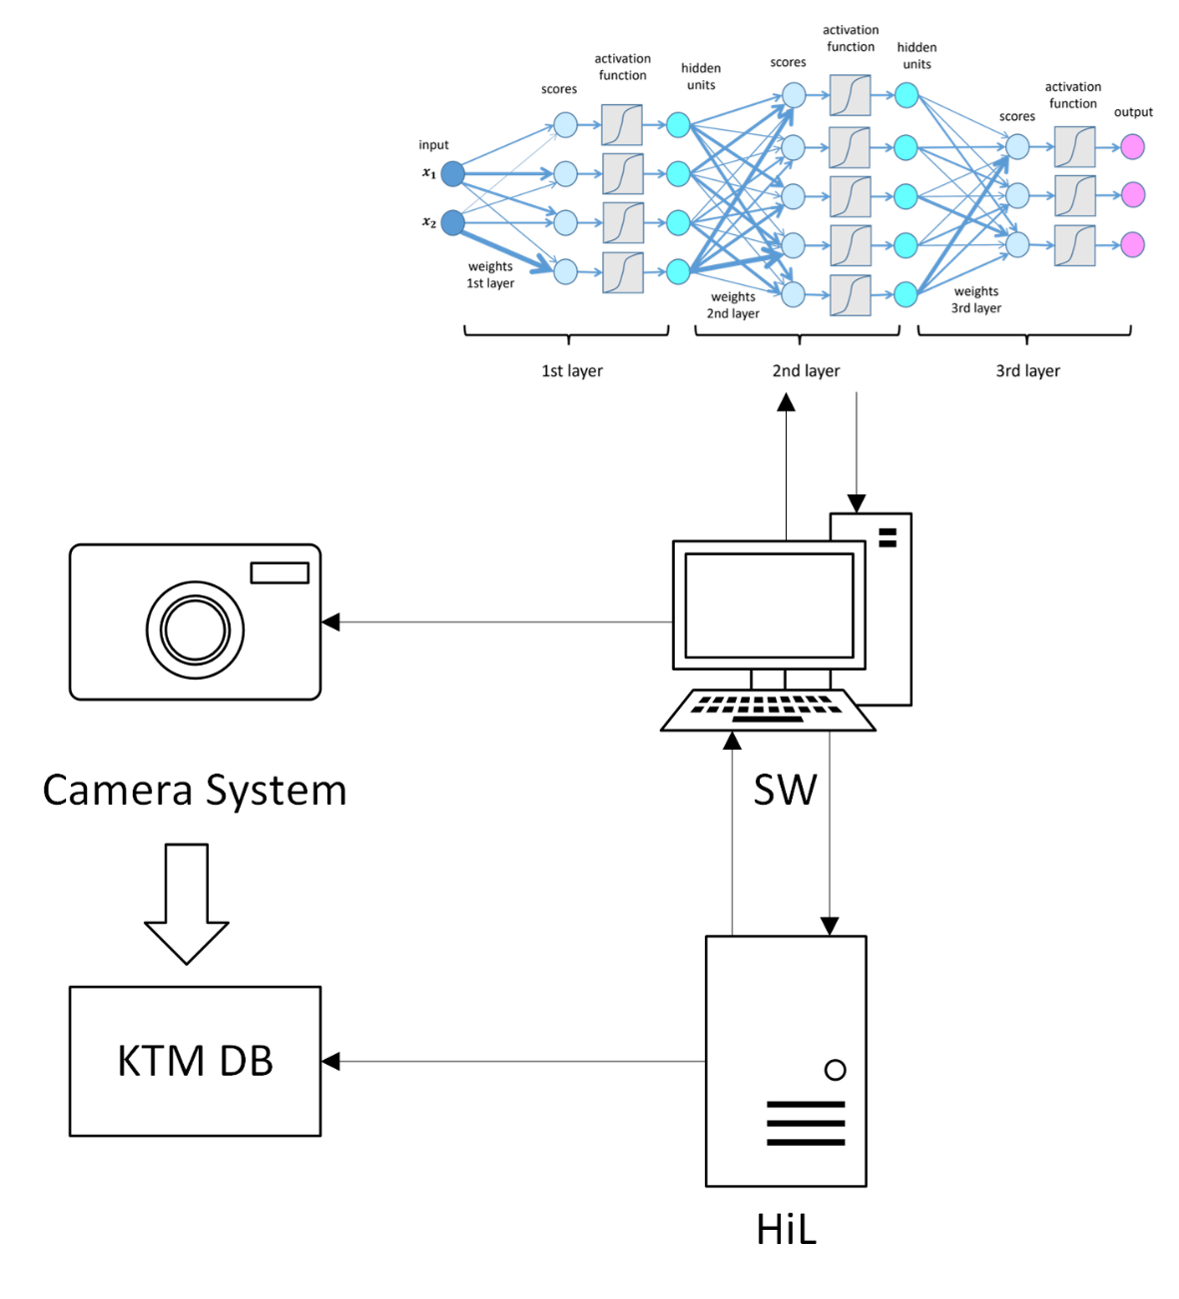
\includegraphics[width=0.6\textwidth]{Figures/Project_overview.png}
    \caption{Project overview diagram.}
    \label{proj_overview}
\end{figure}

The methodology used in this project is divided into three main milestones. The first milestone focuses on setting up the test environment. This includes selecting a suitable \gls{cs}, implementing light control, and integrating the \gls{hil} system. The goal is to create a fully functional closed-loop setup that can later be used to integrate the model and run detection tests.

The second milestone involves preparing a \gls{ds} in an automated way using Photoshop files. It includes image annotation, preprocessing, and augmentation to improve model generalization. Moreover, this stage includes training the selected \gls{od} model using the \gls{ds} and testing its performance on images captured from the \gls{cs}.

The third milestone is focused on integrating the trained \gls{od} model with the \gls{sw}. This \gls{sw} is responsible for synchronizing with the \gls{hil} system to carry out the complete validation cycle.


\section{Test Setup}
The test setup is an important part of the project as it provides the environment in which the \gls{db} will be tested and evaluated. The setup includes the selection of a suitable \gls{cs}, light control and the integration of a \gls{hil} system. The goal of this milestone is to develop a complete closed loop setup that is ready to integrate the model and run the detection process in the test environment. The following sections provide an overview of the test setup, including the \gls{cs}, light control and \gls{hil} integration.

\subsection{Camera System}
To evaluate the \gls{db}, the test setup relies on the \gls{cs} to capture clear and accurate images. It should be able to capture high-resolution images with a wide \gls{fov} to ensure that all relevant dashboard elements are clearly visible in each frame. Since a dedicated light control system is used to ensure consistent lighting conditions, the camera does not need to be highly sensitive to light variations. This light control approach will be explained in more detail later in this chapter. Moreover, as the \gls{db} remains stationary during testing, motion blur sensitivity is not a critical requirement.

Since a \gls{cs} was already available at KTM, it was recommended to use the existing system for this project. The chosen \gls{cs} is a high-resolution camera provided by Cognex, a company specializing in industrial grade \gls{cs}. This camera can capture images at a resolution of up to 12 megapixels (4096 × 3000), which is sufficient for the \gls{od} model to accurately detect and classify dashboard elements \cite{Cognex_Camera}. Figure~\ref{Cognex_Camera} shows the \gls{cs} used in the test setup.

\begin{figure}[!htb]
    \centering
    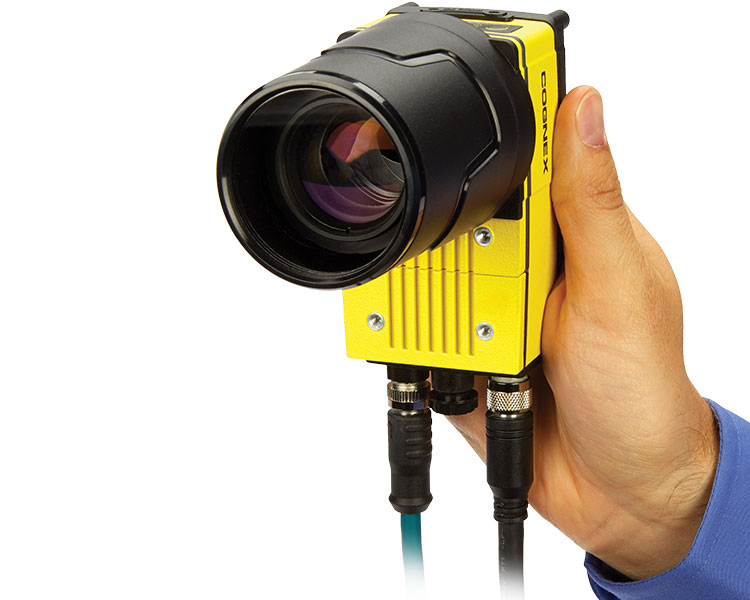
\includegraphics[width=0.5\textwidth]{Figures/In-Sight 9000 in hand.jpg}
    \caption{Cognex \gls{cs} used in the test setup \cite{Cognex_Camera}.}
    \label{Cognex_Camera}
\end{figure}

Additionally, Cognex \gls{cs} is able to communicate with external devices over Ethernet networks or serial port connections using various protocols. This allows smooth integration with the \gls{sw}, enabling reliable image capture and retrieval using \gls{telnet} and \gls{ftp} protocols through the native mode communication. The Cognex native mode communication protocol is an ASCII-based command system used to remotely control Cognex sensors. It supports communication through custom PC applications, remote serial hosts, or \gls{telnet} over Ethernet. The protocol includes two types of commands: basic (short, two-character commands) and extended (with additional functionality). When a command is sent, the sensor processes it and replies with an ASCII response. Set commands return 1 for success, 0 for unrecognized commands, or a negative number for failure, while get commands return specific values based on the request \cite{Cognex_Com}. In this project the basic comands are sufficient since it is only required to trigger an image and retrieve it. 

Set Event command was chosen to trigger an image capaturing event, it triggers a specified event through a basic native mode command. A python code was created to trigger an image capturing using this command via \gls{telnet} and then retrieve it using \gls{ftp}, the flow chart of the code is shown in figure \ref{Image_capture_code}. The Set Event command is SE8 according to Cognex documentation \cite{Cognex_Com}.

\begin{figure}[!htb]
    \centering
    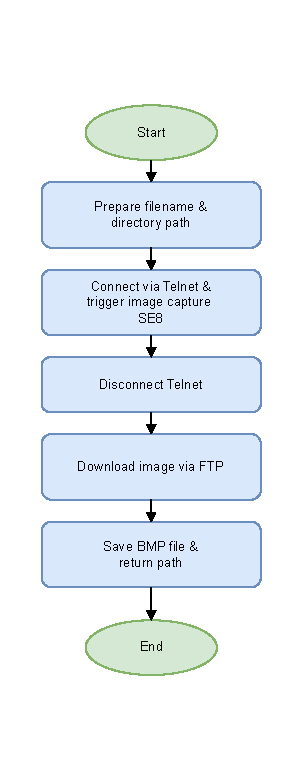
\includegraphics[width=0.3\textwidth]{Figures/diagrams/Image_Capturing.pdf}
    \caption{Process overview of image acquisition from a Cognex sensor using \gls{telnet} triggered capture and \gls{ftp} file retrieval.}
    \label{Image_capture_code}
\end{figure}

Error handling and fallback scenarios were considered when designing the function for further integration in the complete architecture. Later in this chapter this function will be used as a first step when the \gls{hil} requests an image analysis from the standalone \gls{sw}.

\subsection{Light Control}
To ensure that the \gls{cs} captures images under controlled optimum lighting conditions, a light control system is an essential part of the test setup. This is important for the performance of the \gls{od} model, as variations in lighting can significantly affect the quality of the detection model. The light control system should prevent any external light sources from interfering with the captured images, this is important to ensure that no glare or reflections are present in the images, which can lead to false detections or misclassifications.

KTM uses a light control system that consists of a box with aluminum frame and black walls to prevent any external light or light reflections. The box is equipped with a set of LED lights that can be adjusted to provide the desired level of illumination. The lights are positioned to ensure that the entire \gls{fov} of the camera is evenly illuminated, and they can be controlled remotely to adjust the brightness and color temperature as needed. This allows for complete control over the lighting conditions during the testing process, ensuring that the images captured by the camera are of high quality and suitable for the \gls{od} model. Figure \ref{LightControl} shows the light control system used in the test setup.

\begin{figure}[!htb]
    \centering
    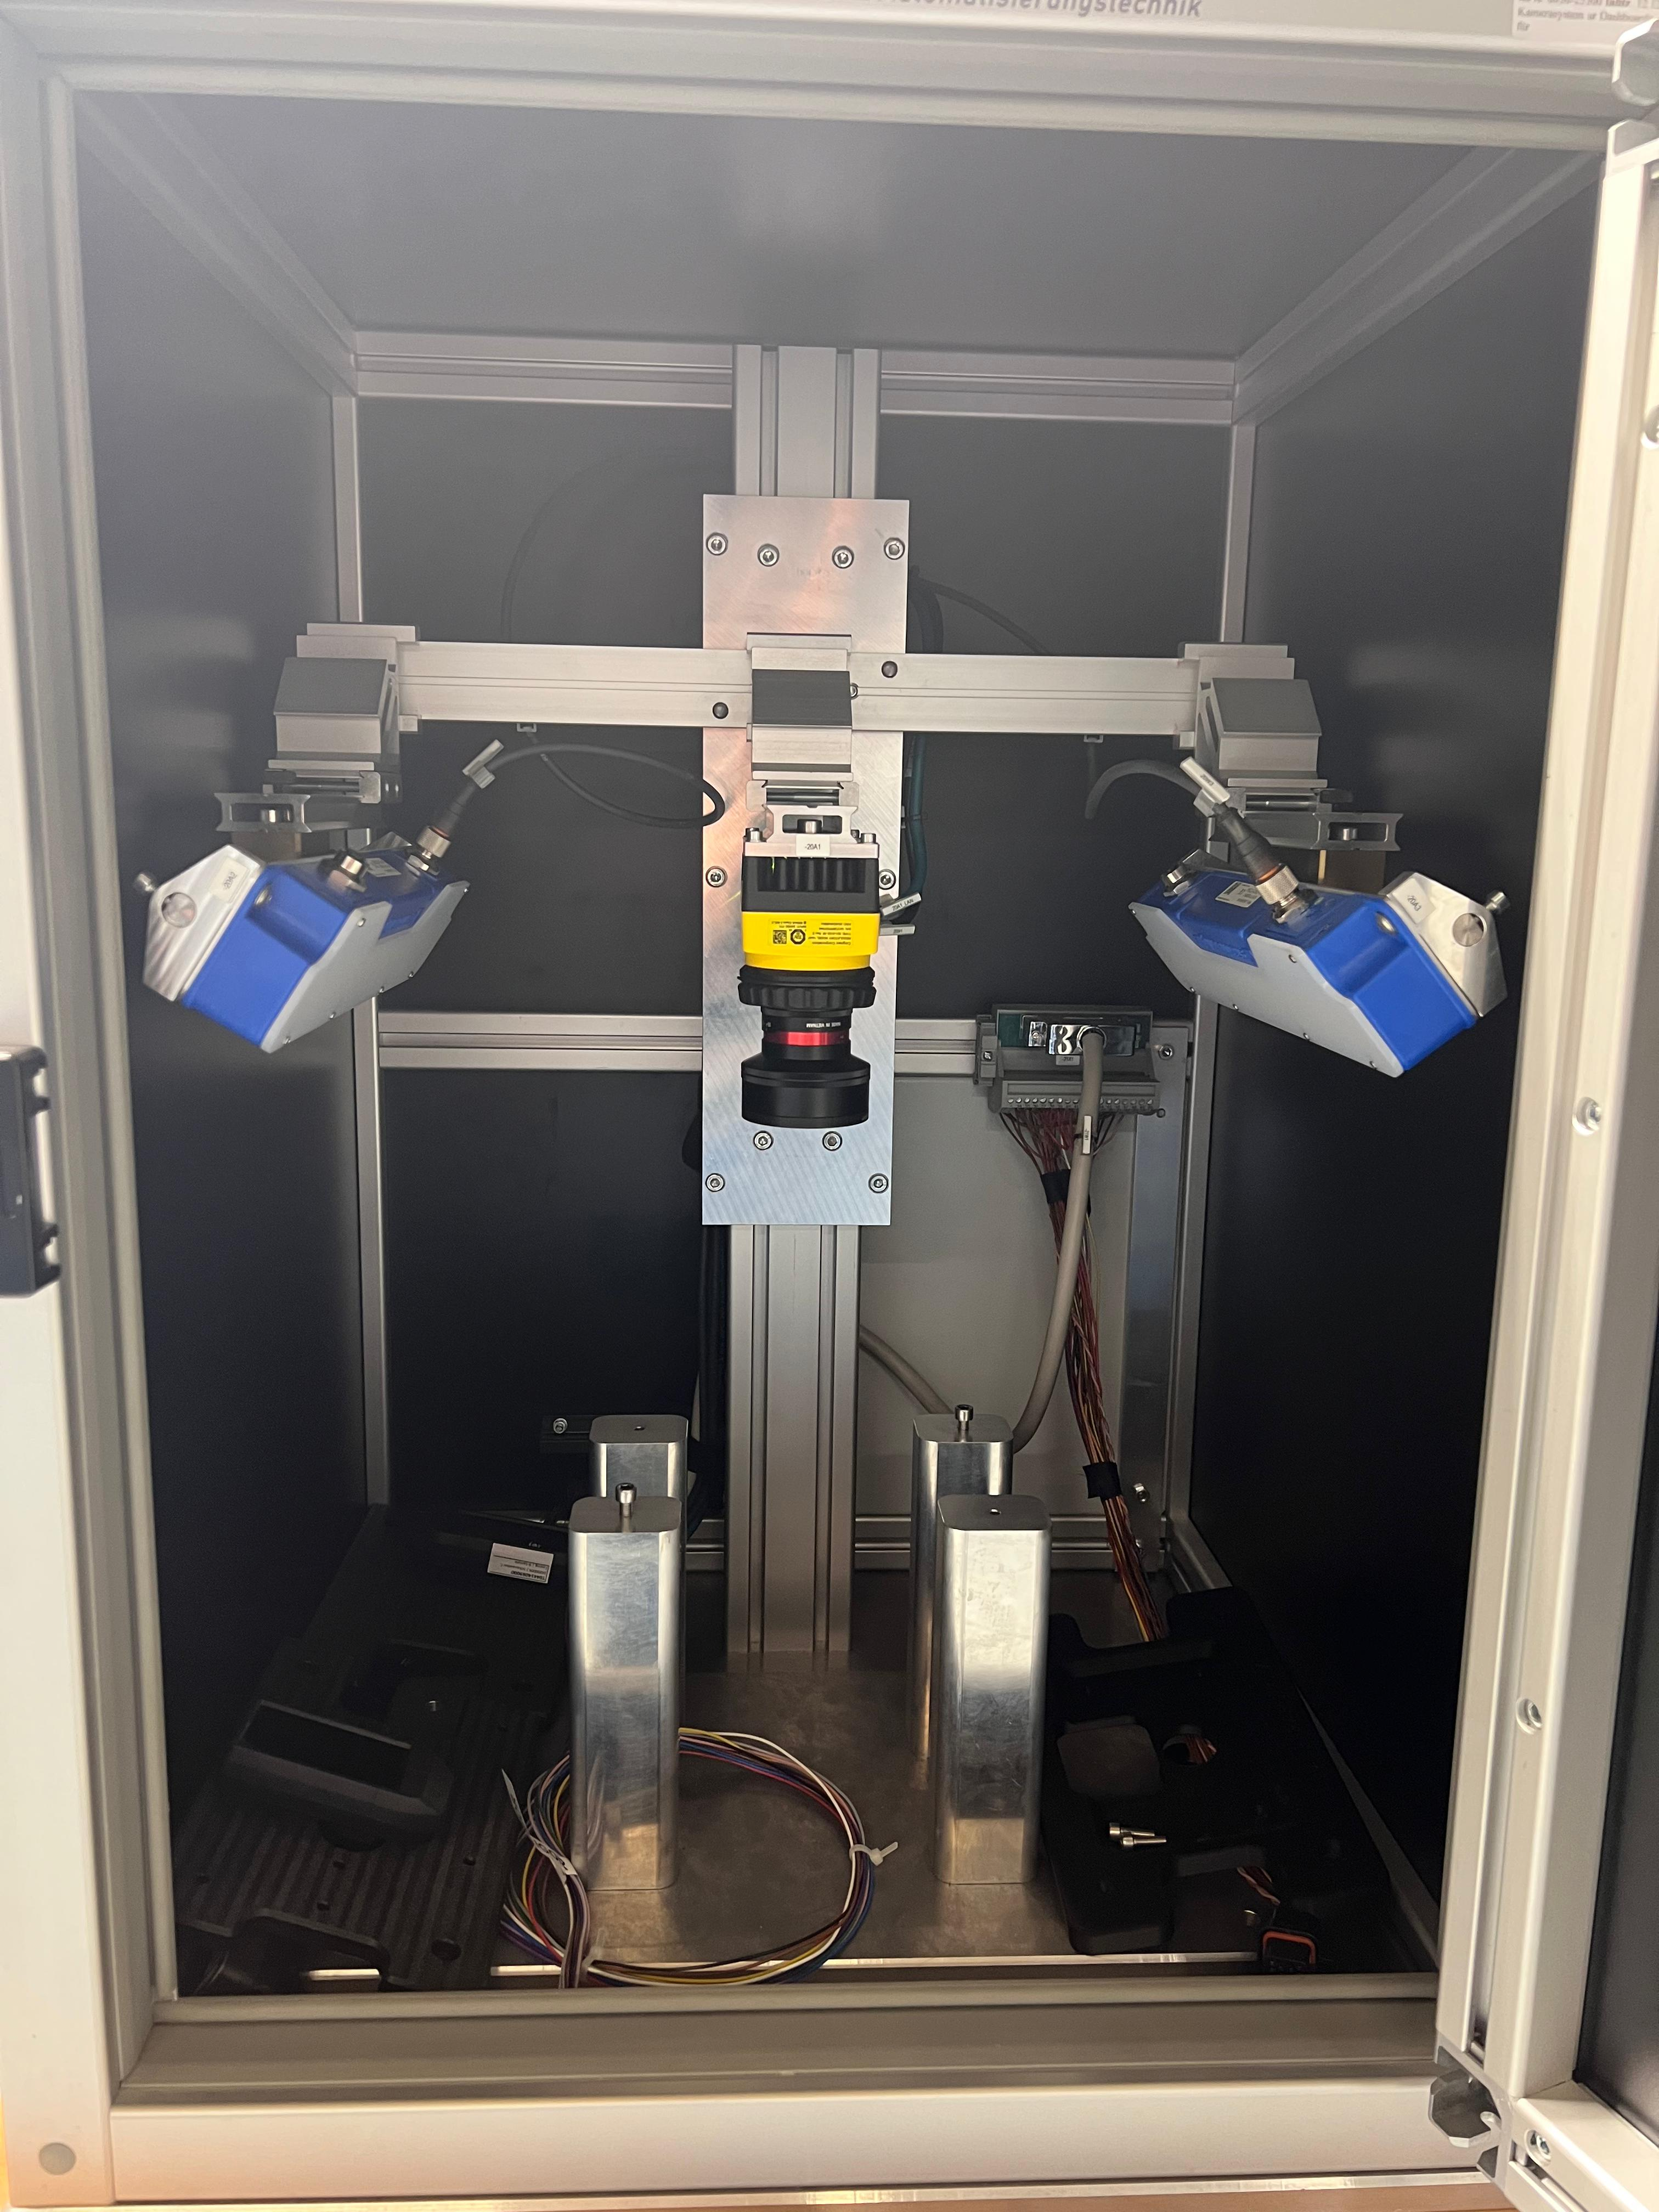
\includegraphics[width=0.6\textwidth]{Figures/Light_Control_Box.jpg}
    \caption{Light control system used in the test setup.}
    \label{LightControl}
\end{figure}

The box provides a mounting structure for the \gls{cs} to ensure that the \gls{cs} is positioned correctly and securely during the testing process. The mounting structure allows easy adjustment of the camera position and angle to ensure that the entire \gls{db} is captured in the images. Figure \ref{Camera_Mounting} shows the \gls{cs} mounted inside the light control box. The light control box also includes a mounting structure for the the \gls{db} to ensure that the distance between the \gls{cs} and the \gls{db} is consistent. Figure \ref{db_Mounting} shows the \gls{db} mounted in a secure way in the light control box. Additionally, a cable inlet is provided to allow for the connection of the \gls{cs} and the \gls{db} without compromising the light control system.

\begin{figure}[!htb]
    \centering
    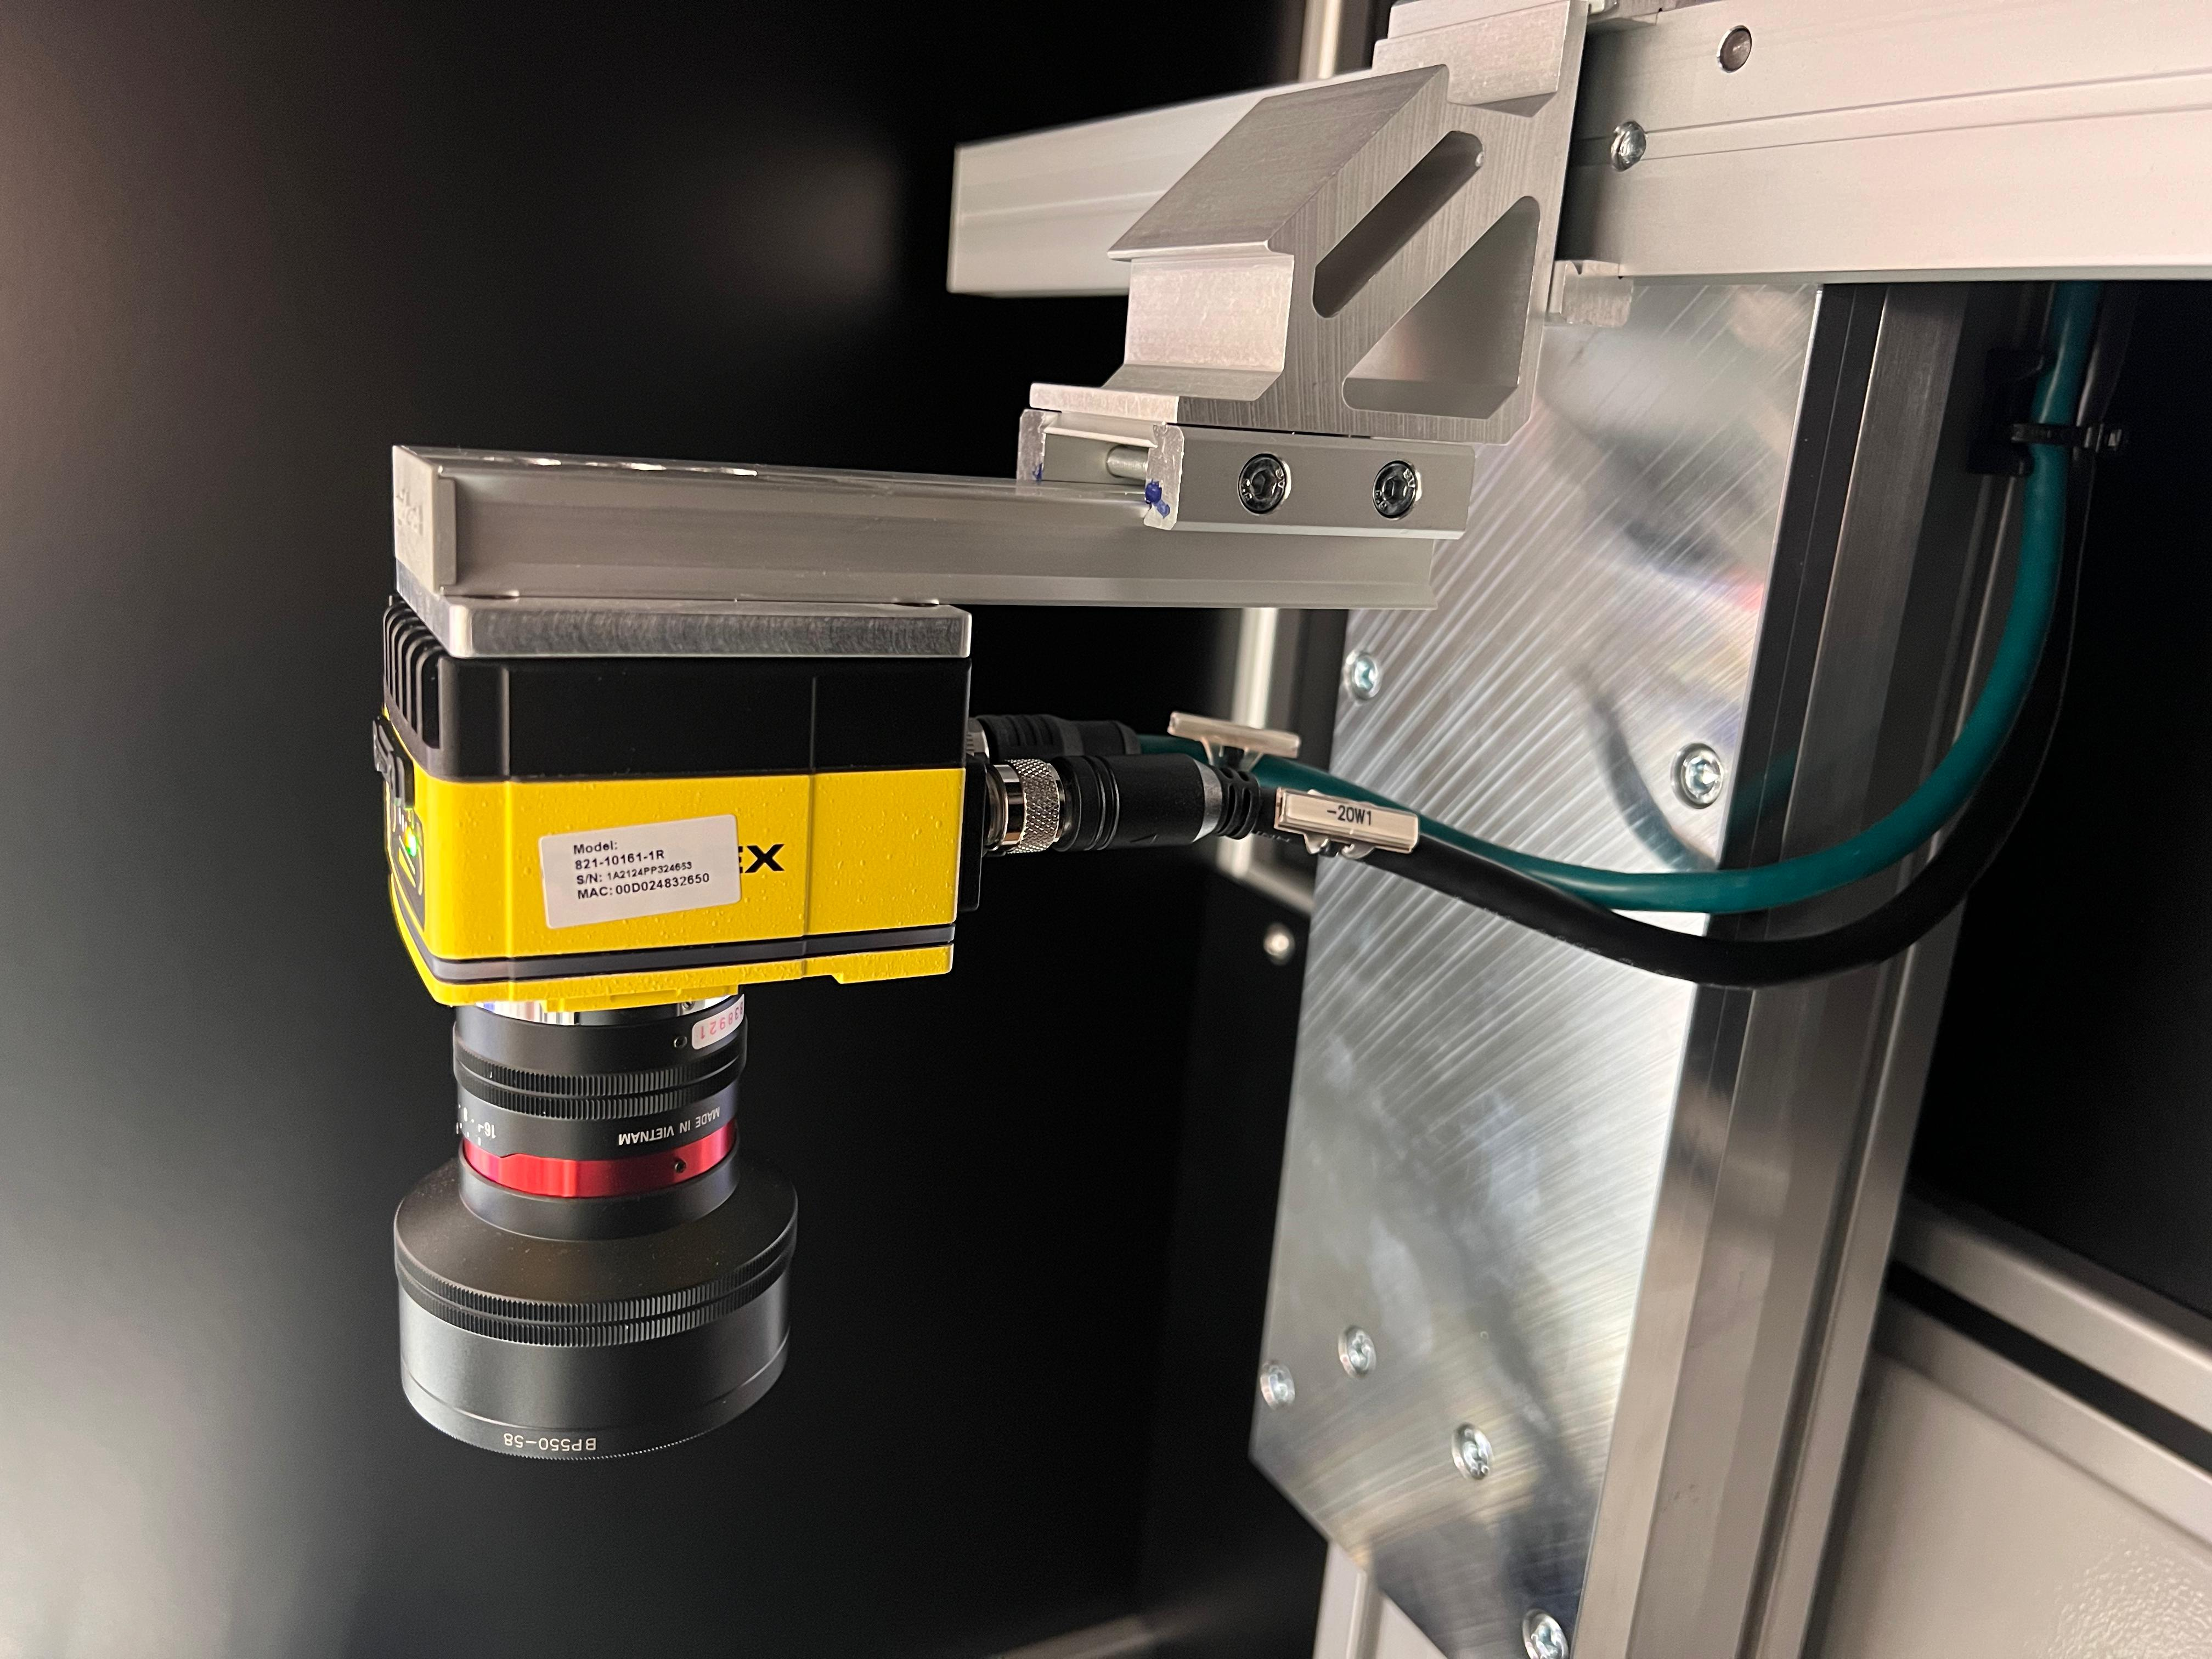
\includegraphics[width=0.6\textwidth]{Figures/Camera_Mounting.jpg}
    \caption{\gls{cs} mounted inside the light control box.}
    \label{Camera_Mounting}
\end{figure}

\begin{figure}[!htb]
    \centering
    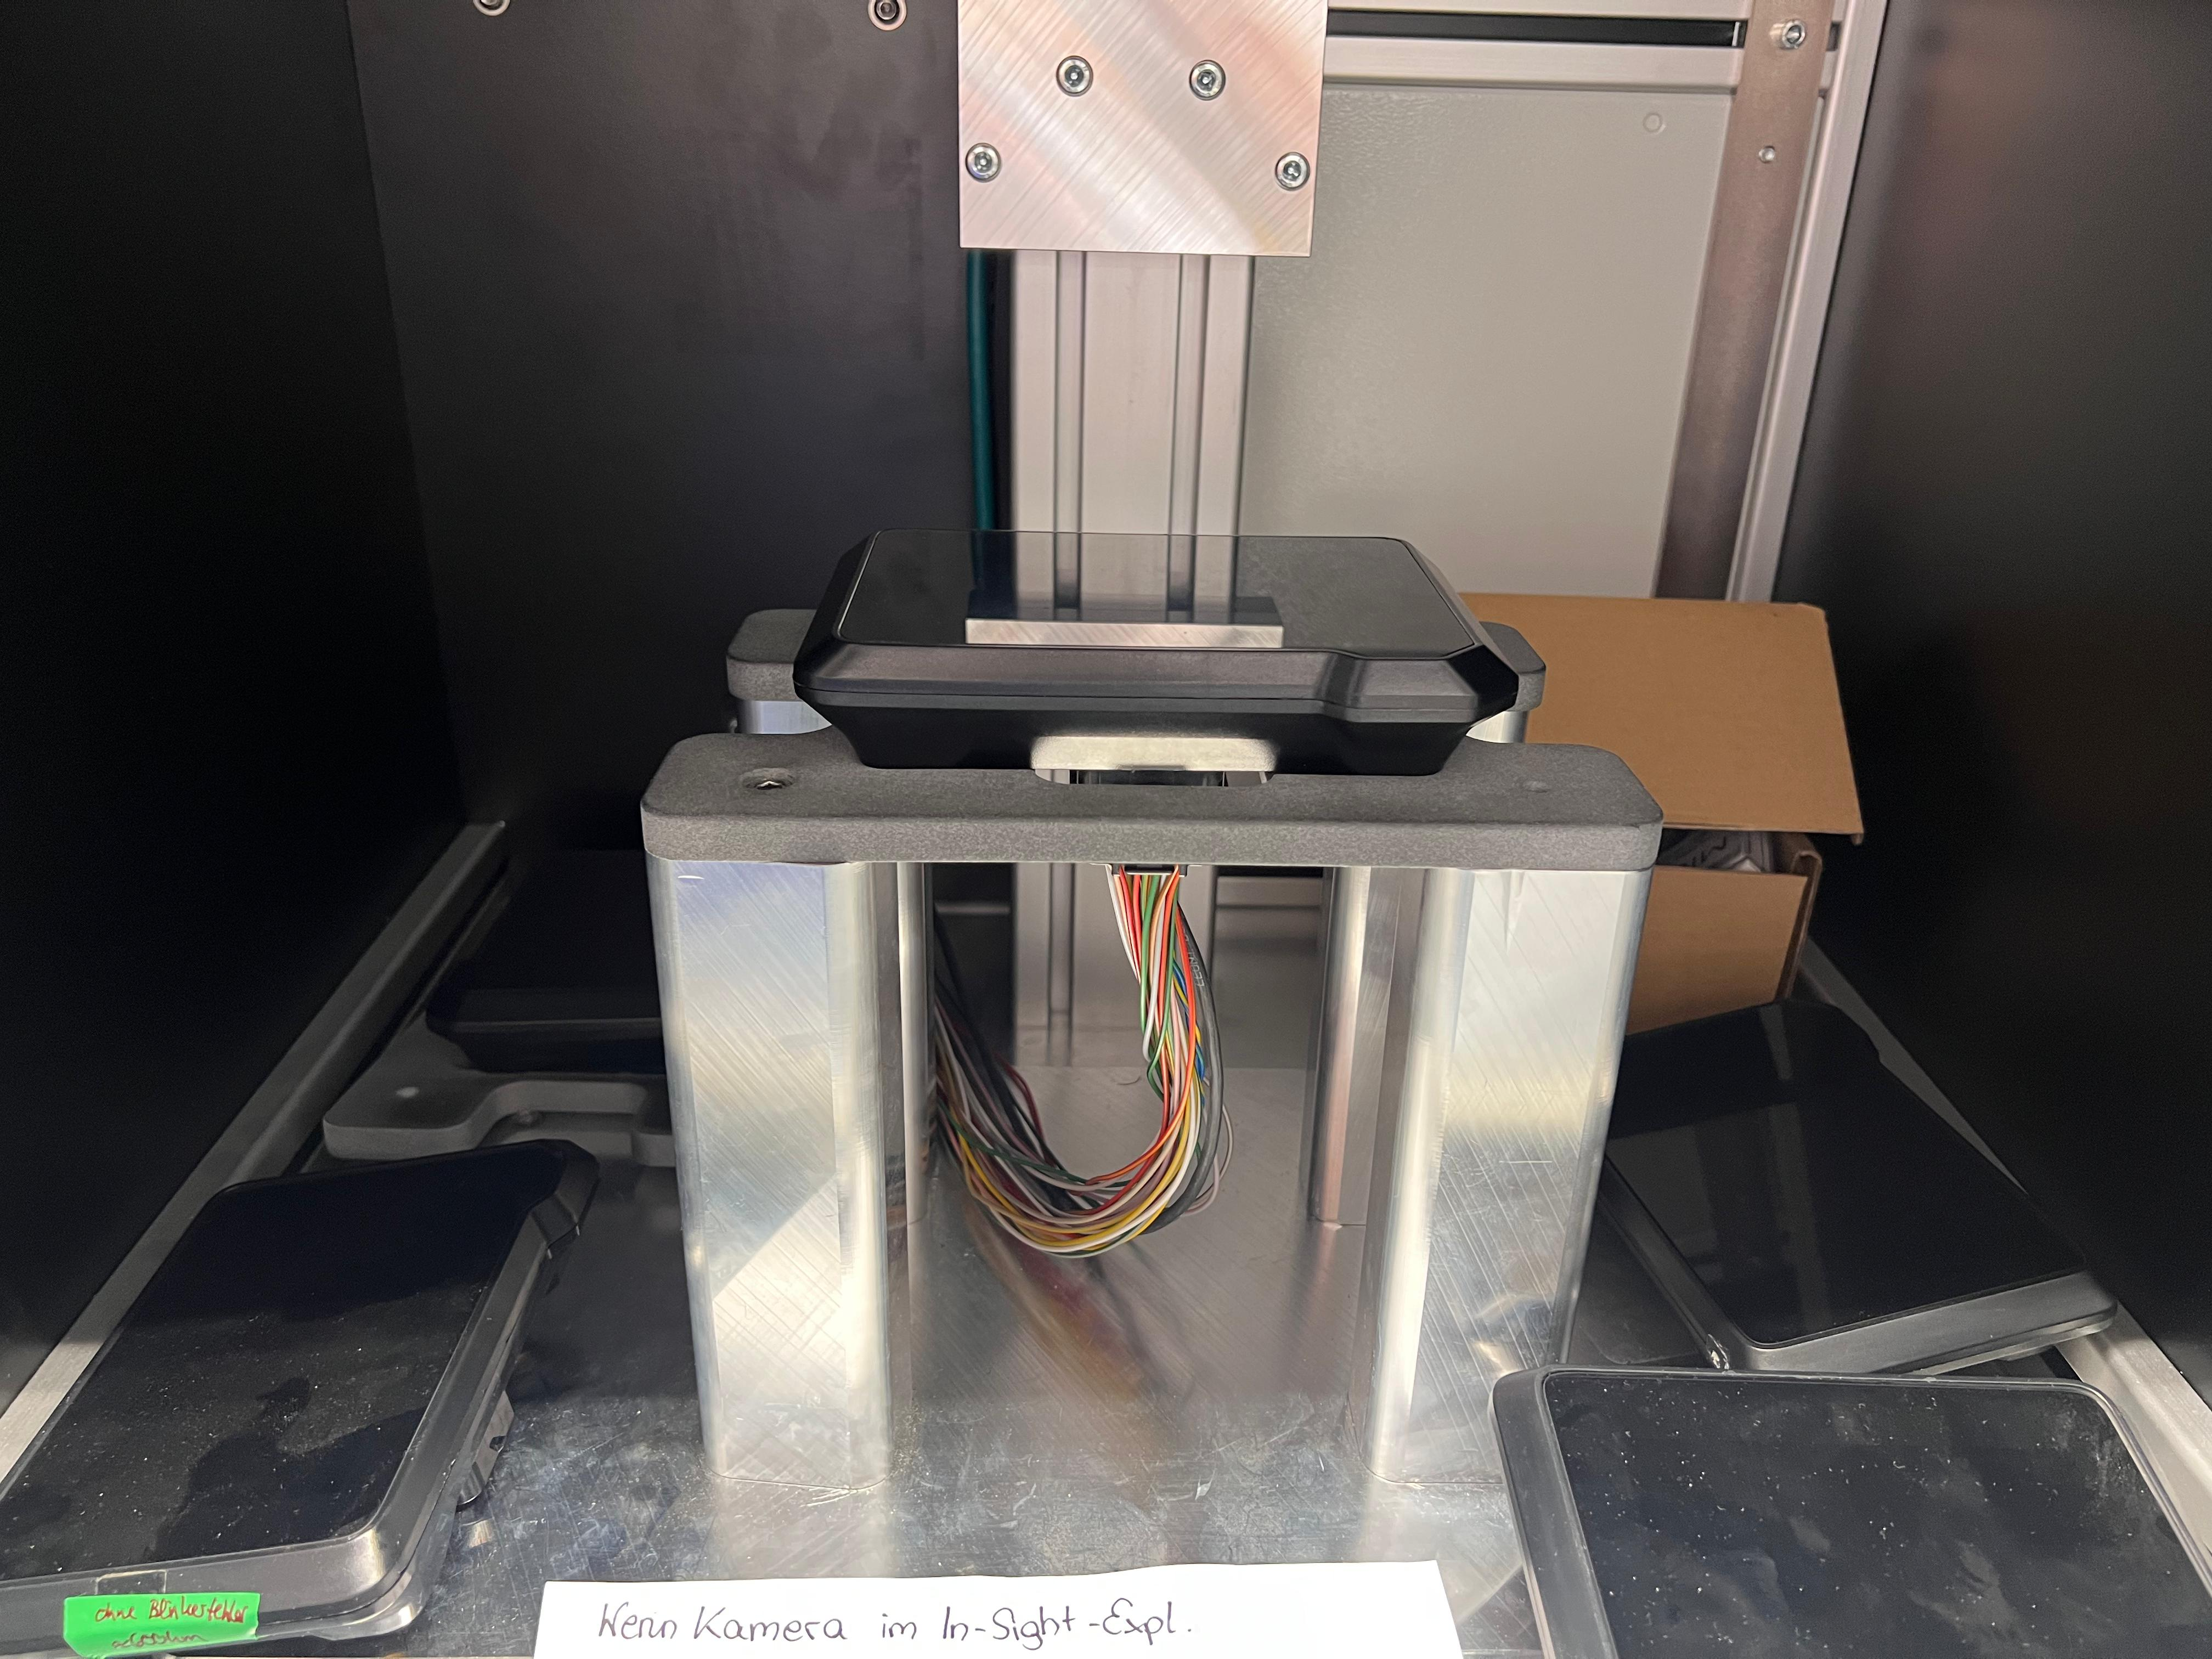
\includegraphics[width=0.6\textwidth]{Figures/db_mounting.jpg}
    \caption{\gls{db} mounted inside the light control box.}
    \label{db_Mounting}
\end{figure}

\subsection{Hardware In The Loop System Integration}
As mentioned earlier, the \gls{hil} system controls the entire test process. Therefore, it is essential to establish a smooth and reliable integration between the \gls{hil} and the other systems involved in testing. For this project, the Vector \gls{hil} was chosen, as it is already available at KTM and provides a comprehensive suite of software tools. These tools offer flexibility in building test cases using different approaches, ranging from simple sequences to more advanced testing scenarios.

Additionally, the Vector toolchain supports the .NET framework for developing test cases. This is particularly useful, as it includes all the standard libraries needed for enabling HTTP communication between the \gls{hil} and external systems.

Moreover, since the standalone \gls{sw} is developed in Python and the systems are designed to communicate synchronously, Flask was chosen as the main framework to manage communication between the components. Compared to other frameworks like gRPC, which require protocol buffer definitions and additional dependencies, Flask provides a much simpler setup. This makes it easier to integrate into the \gls{hil} development environment without the need to add external libraries or tools, resulting in a lightweight and maintainable solution.

To achieve the goal of the first milestone, which is to develop a closed-loop test setup that is ready for model integration, it was decided to create a single Python function that handles the entire process. This function combines image acquisition, image analysis, and results comparison into one streamlined workflow. As a result, a Flask server can be built to expose just this single function, which is then triggered once by the \gls{hil}. The function executes the complete sequence and returns the final results. 

To support this approach, the image acquisition process was encapsulated in a Python function called \texttt{capture\_and\_save\_image(filename)}. As explained earlier, this function captures an image, saves it under the given filename in the designated directory, and returns the full path to the saved image.

In preparation to complete the first milestone, a second placeholder function was created: \texttt{start\_image\_analysis(image\_path)}. This function will later be developed to load the image from the provided path and use the trained model to detect all relevant \gls{db} elements. It will then store these elements in a list and return it for further evaluation.

The third function, \texttt{compare\_results(detected\_elements, filename)}, takes the list of detected elements and the filename as inputs. The filename provided by the \gls{hil} includes the elements that needs to be verified. This function searches the list for the specified elements and returns \texttt{True} if the elements are found or \texttt{False} otherwise.

Finally, all three functions are called in the mentioned sequence within a main function called \texttt{analyze\_image(filename)}. This function includes error handling and returns \texttt{1} if the comparison passes, \texttt{0} if it fails, and an error message if something goes wrong to provide clear feedback to be logged by the \gls{hil}. Figure \ref{analyze_image} provide a cleare schematic for the process flow of the main function.


\begin{figure}[!h]
    \centering
    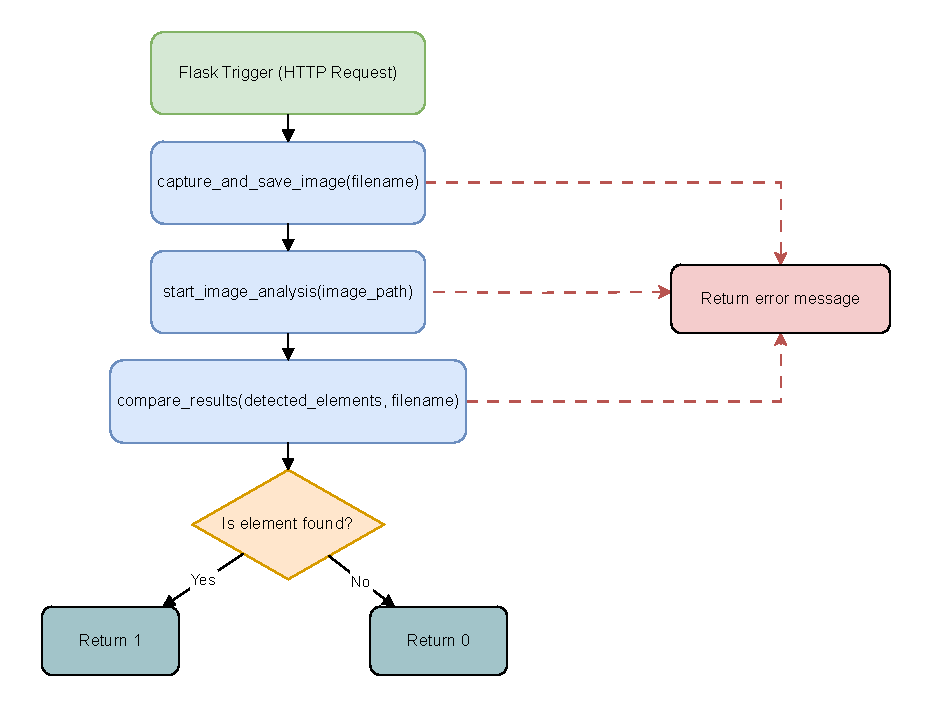
\includegraphics[width=0.7\textwidth]{Figures/diagrams/analyze_image.pdf}
    \caption{Process flow of the \texttt{analyze\_image(filename)} function.}
    \label{analyze_image}
\end{figure}

Once the main function was ready, the next step was to configure the network environment in which all devices would operate. Since all systems were connected to the same subnet, as shown in Figure \ref{Network}, it was possible to host the Flask application on IP address \texttt{192.168.100.50} using the standard Flask port \texttt{5000}. This allowed HTTP requests to be sent in the format: \texttt{http://192.168.100.50:5000/analyze\_image+filename}.

\begin{figure}[!h]
    \centering
    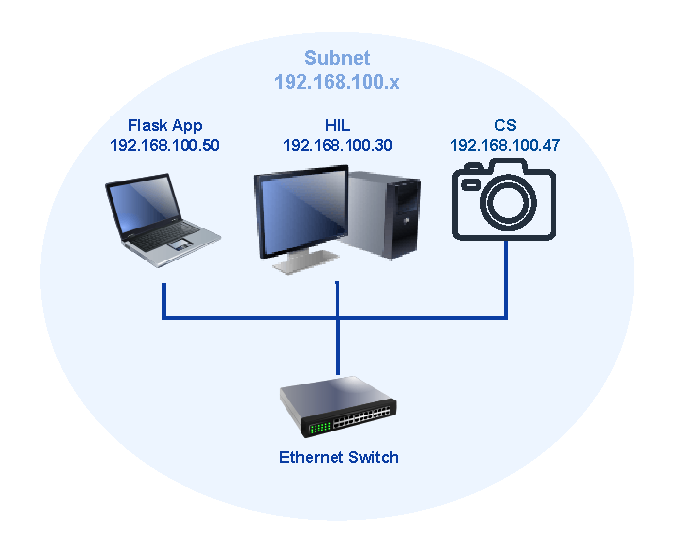
\includegraphics[width=0.7\textwidth]{Figures/diagrams/Network.pdf}
    \caption{Subnet which have all the devices connected on.}
    \label{Network}
\end{figure}

On the \gls{hil} side, a test function was implemented using the .NET framework. This function takes a string input representing the filename, sends an HTTP request to the Flask application and waits for a response. If the response is positive, the test case is considered passed. This modular function can be integrated into any test scenario, making it possible to validate individual \gls{db} frames by simply passing the relevant elements in the string filename.

The final step of the first milestone involved creating a test case that activates a combination of \gls{db} icons to simulate a real dashboard frame. This was implemented using the test table in vTESTstudio, as shown in Figure~\ref{Test_Case_1}. In this test case, four dashboard icons are turned on via CAN messages, followed by a call to the test function that sends the HTTP request to the Flask server. After a short wait, the icons are turned off again.

\begin{figure}[!h]
    \centering
    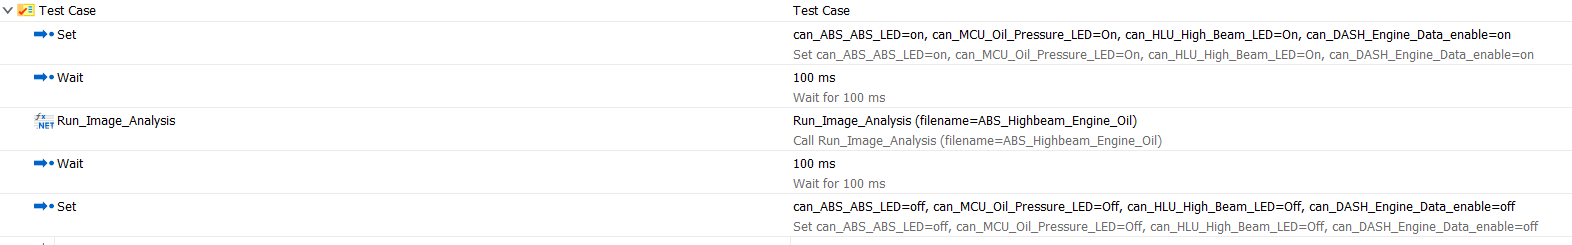
\includegraphics[width=0.9\textwidth]{Figures/Test_Case_1.png}
    \caption{Example test case that turns on four \gls{db} icons, running analysis and turning them off again.}
    \label{Test_Case_1}
\end{figure}

This step is a key foundation for the entire project workflow, as it demonstrates how any \gls{db} frame can be tested in the same structured way. With this setup in place, the system is now fully prepared to integrate the trained model and run real detection tests.

The output of this milestone is an image of the \gls{db}, saved on the server computer and ready for analysis. An example of this captured image is shown in figure \ref{DB_4_raw}.

\begin{figure}[!h]
    \centering
    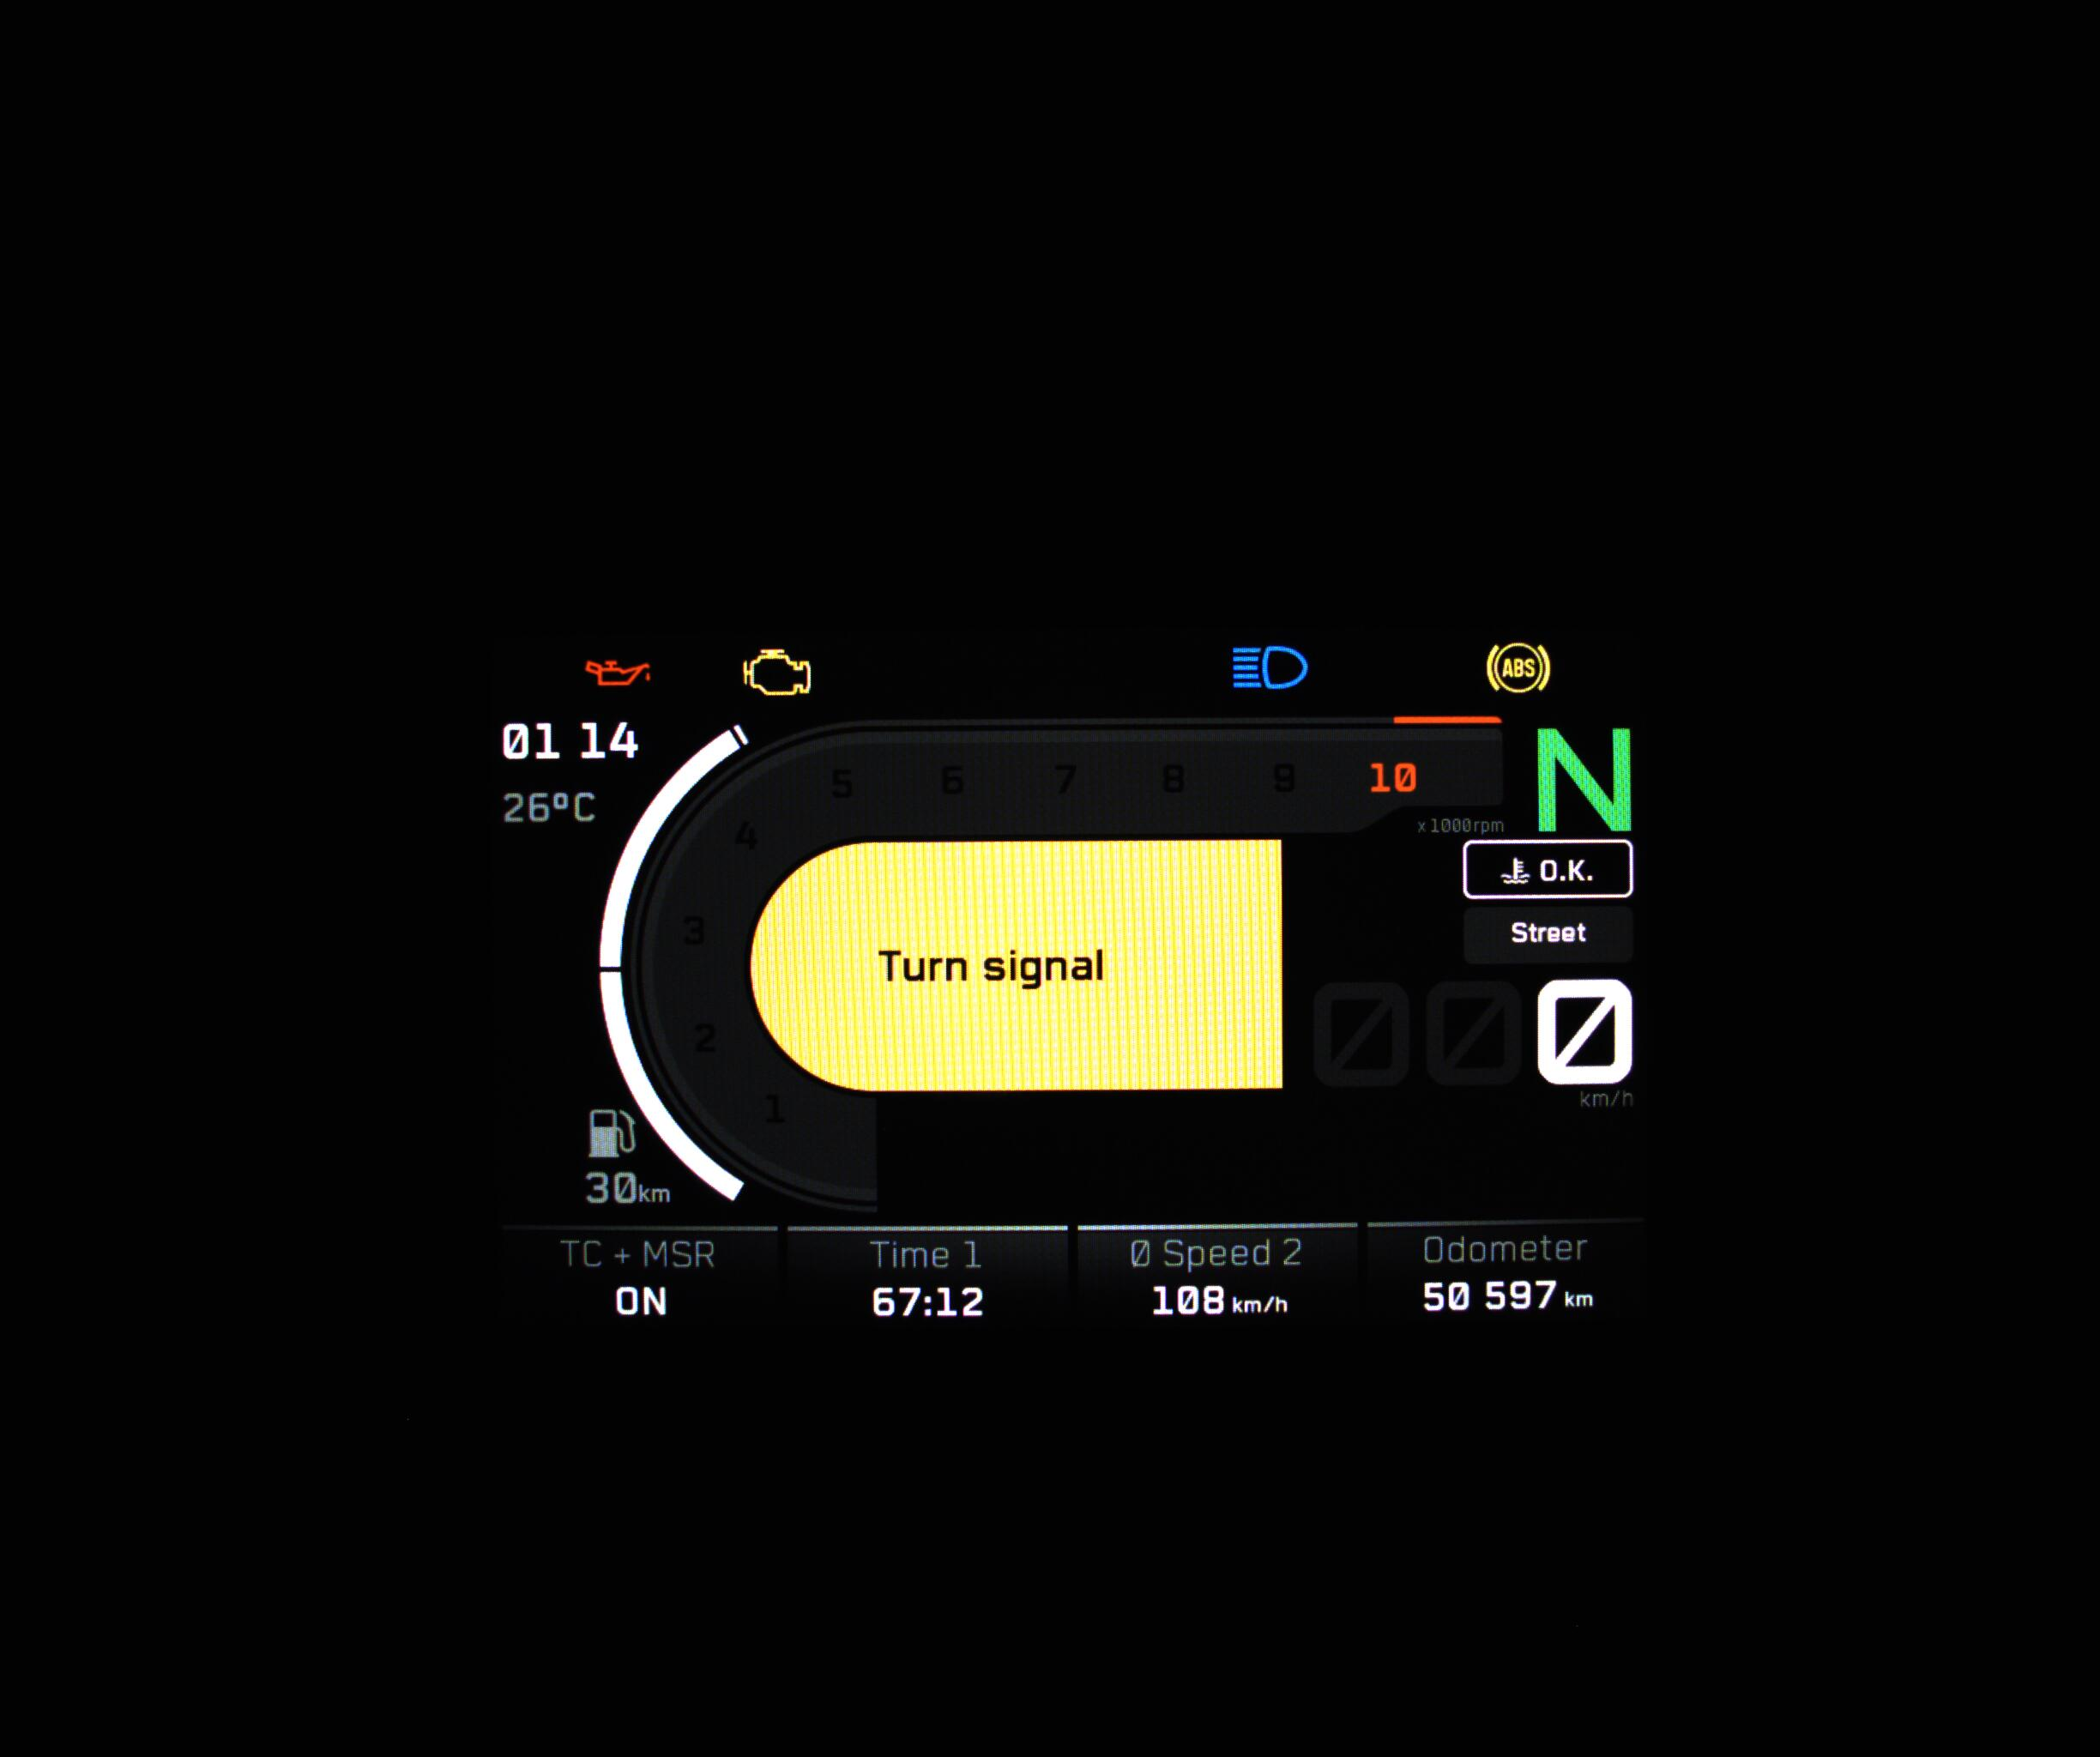
\includegraphics[width=0.5\textwidth]{Figures/4.png}
    \caption{Example \gls{db} camera image containing the four required icons.}
    \label{DB_4_raw}
\end{figure}


\section{Object Detection Model}
In this milestone, the main focus is on training a \gls{dl} model that can reliably and accurately detect \gls{db} elements. Due to time constraints, the project concentrates on a single class of \gls{db} elements, specifically the telltale icons. This category includes a set of ten icons that are selected for validation.

To develop a working model, the process begins with preparing a suitable \gls{ds}. This includes \gls{dc}, images annotation, performing preprocessing steps and applying augmentation techniques to improve generalization.

Once the \gls{ds} is ready, the training process begins. This involves selecting an appropriate model architecture from those described in the technical background chapter, training it on the prepared training \gls{ds} and evaluating its performance using the validation and test \gls{ds}. The final evaluation is performed using real camera images captured by the selected \gls{cs} to ensure the model performs well under actual testing conditions.

\subsection{Dataset Preparation}
The \gls{ds} preparation process consists of several steps, as outlined in the previous chapter. The first step is \gls{dc}. Since the \gls{db} needs to be validated during the development phase, it is essential to maintain a high level of privacy and control. Therefore, a private \gls{dc} approach was chosen for this project to ensure that the training images are both relevant and secure.

At this stage, the actual \gls{sw} is still under development. However, Photoshop design files of the \gls{db} were already available. Based on these files, the training data was collected by exporting images that included all possible combinations of the selected telltale icons using a single background frame. Although it is possible to use different background frames, only one was selected for simplicity. This frame includes the most complex colors and visual elements to help train the model under the most challenging visual conditions.

Using this setup, a total of one thousand and twenty four unique images could be generated. However, exporting this number of images manually is time consuming and labor intensive, which would be impractical in a real development environment. To address this, Adobe Photoshop built in automation capabilities were used. A JavaScript script was developed to automate the process of hiding and showing the telltale icon layers in the correct sequence and exporting each image. The script also assigned each image a filename that includes the names of the visible icons. For example, an image showing \gls{abs} and engine icons would be saved as \texttt{ABS\_Engine.png}. This naming format simplifies the annotation process, which will be discussed further in this section.

After collecting the data, the annotation process begins. As mentioned in the previous chapter, this step is often the most time consuming and most prone to error. For that reason, automating it is highly beneficial, as it helps avoid spending weeks of company resources manually drawing bounding boxes around important icons.

Since the \gls{ds} was created by exporting images from Photoshop files, the positions of the icons and other assets are fixed whenever they are present. Additionally, the visible icons are listed in the filename, as described earlier. By combining these two factors, it became clear that a Python script could be used to automate the annotation process. The script reads the icon names from the filename, retrieves the corresponding predefined positions, and generates an annotation file for that specific image. The output is saved in the labels directory using the same filename as the image to ensure that it can be easily matched later during training.

For example, if an image contains the icons for oil, engine, and \gls{abs}, the script creates a text file like the one shown in Figure \ref{oil_engine_abs_txt}. Each line in the file corresponds to a detected object and includes the class identification (such as six for oil and zero for \gls{abs}) in the first column, followed by the values for the bounding box center coordinates (x, y), then width and height in the last two columns. The annotation format depends on the chosen architecture which will be discussed further in this chapter. However, once one format was created, it could be transformed easily in differant formats if differant architecture is chosen later. At this stage, \gls{yolo} text file format was chosen because it is the easiest and most likely to be used.

\begin{figure}[!h]
    \centering
    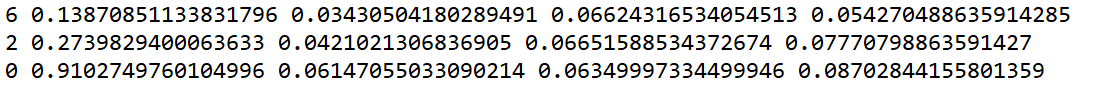
\includegraphics[width=0.7\textwidth]{Figures/Oil_Engine_ABS.png}
    \caption{Example of a \gls{yolo} annotation text file for an image containing oil, engine and \gls{abs} icons}
    \label{oil_engine_abs_txt}
\end{figure}

After the annotation of the \gls{ds} was completed, it was important to ensure that the image size matched the expected input dimensions of the selected model architecture. Most modern architectures typically accept input images of size $640 \times 640$.

Additionally, the images exported from the Photoshop files are of much higher quality and clarity compared to those that will be captured by the \gls{cs}. This difference in quality can cause the model to overfit on the training \gls{ds} and makie it less effective at detecting icons in real test scenarios.

To address these issues, image preprocessing techniques such as resizing are necessary to match the model input size. Furthermore, image augmentation techniques like random rotation and the addition of random noise help reduce the artificial sharpness of the training images, allowing the model to generalize better.

One of the main challenges in applying such techniques is the need to adjust the bounding boxes accordingly after transformations. However, modern tools such as Roboflow solve this problem efficiently. Roboflow is a platform that supports the management, annotation, augmentation and export of \gls{ds} for training \gls{ml} models. It can apply preprocessing and augmentation steps while preserving the correct bounding box locations for each asset. In addition, it provides export options in various formats compatible with widely used architectures. Finally, figure \ref{DS_Prep} gives a summary on the whole \gls{ds} preparation process with key takeaway points of it.

\begin{figure}[!h]
    \centering
    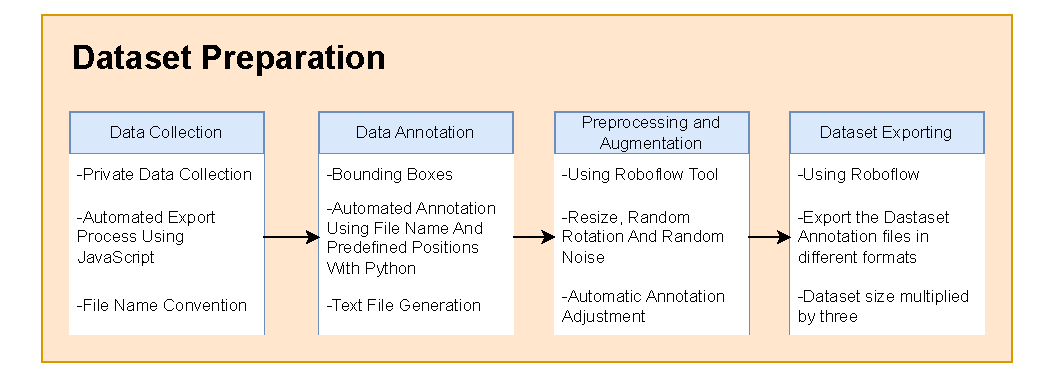
\includegraphics[width=1\textwidth]{Figures/diagrams/DS_Prep.pdf}
    \caption{A summary on the \gls{ds} preparation process.}
    \label{DS_Prep}
\end{figure}

\subsection{Model Training}
After completing the preparation of the \gls{ds}, the process of selecting and training the model begins. As mentioned in the technical background chapter, the two main types of detectors to choose from are one stage detectors and two stage detectors. Since the new generation of KTM \gls{db} includes many animations that will need to be tested in the future, it was important to consider scalability when choosing the detector. For that reason, a one stage detector was selected, even though the current \gls{db} version only involves static frames.

Among the available options, the \gls{yolo}v11 detector was found to be suitable, as it demonstrates strong performance, as shown in Figure \ref{yolo_comparison}. \gls{yolo}v11 provides an excellent balance between inference speed and accuracy across various model sizes. All \gls{yolo}v11 variants, ranging from nano to extra large, outperform previous \gls{yolo} versions and other state-of-the-art detectors in both accuracy and latency, which supports its selection for this study.

The performance of the model is evaluated using the \gls{map} metric. Specifically, the \textit{\gls{map}}$_{50-95}^{val}$ score is used, which calculates the average precision across ten different intersection over union thresholds ranging from fifty percent to ninety five percent, in steps of five. This provides a more comprehensive measure of how well the model detects and localizes objects, compared to simpler metrics that use only one threshold.

\begin{figure}[!h]
    \centering
    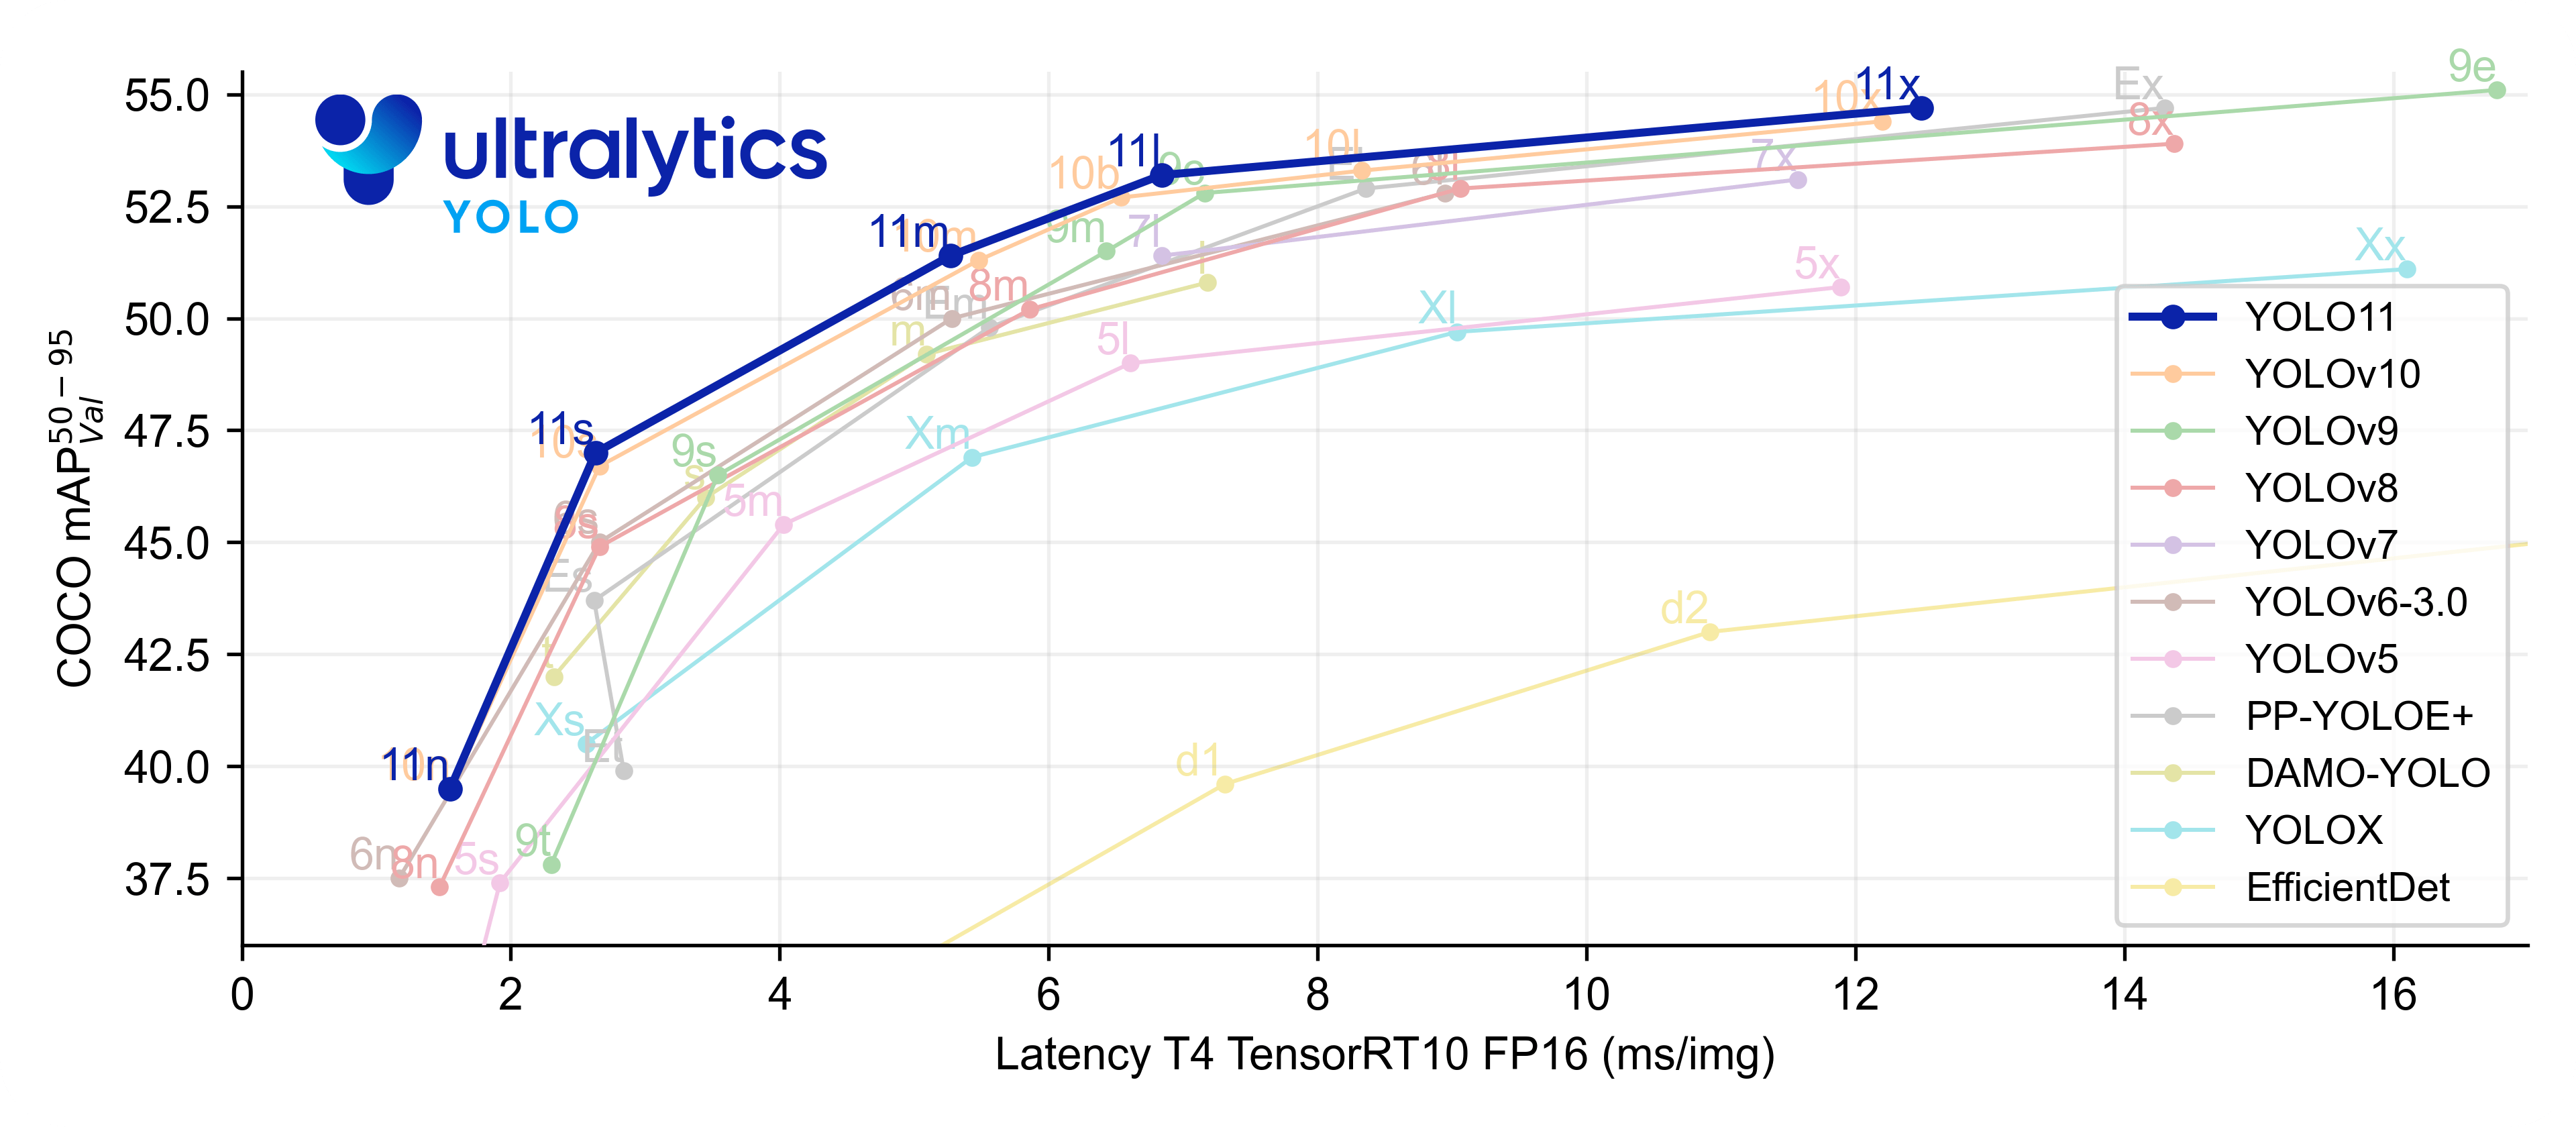
\includegraphics[width=0.95\textwidth]{Figures/performance-comparison.png}
    \caption{Comparison of \gls{od} models in terms of COCO \textit{\gls{map}}$_{50-95}^{val}$ accuracy versus inference latency using TensorRT10 FP16 on an NVIDIA T4 GPU. \gls{yolo}v11 outperforms all previous \gls{yolo} versions and competing models such as PP-\gls{yolo}E+, \gls{yolo}X, and EfficientDet, achieving superior accuracy while maintaining low latency.}
    \label{yolo_comparison}
\end{figure}

Once the model was selected, the next step was to install and train it on the prepared \gls{ds}. \gls{yolo} is developed and provided by Ultralytics, an \gls{ai} company known for building state-of-the-art computer vision tools and models \cite{ultralytics}. The training process is initiated by calling the \texttt{train()} method on the loaded \gls{yolo} model as shown in Listing~\ref{lst:yolo_train}. This method accepts a number of parameters that control how training is performed on the given \gls{ds}. Each parameter is described below:

\begin{itemize}
  \item \texttt{data}: Specifies the path to the dataset configuration file (in YAML format), which defines the locations of the training, validation and testing images, the class names and the number of classes. This file is provided in the exported \gls{ds} folder provided by Roboflow.

  \item \texttt{epochs}: Indicates how many complete passes the model will make over the training dataset. For example, a value of twenty means the model will go through the entire dataset twenty times unless early stopping is triggered.

  \item \texttt{batch}: Sets the batch size, which determines how many images are processed simultaneously during training. A smaller batch size such as eight may be required when GPU memory is limited.

  \item \texttt{imgsz}: Defines the size of the input images. All images are resized to (640 x 640) pixels to standardize the input size and reduce computational load.

  \item \texttt{plots}: When enabled, this parameter generates performance plots such as loss curves and precision-recall graphs at the end of training.

  \item \texttt{verbose}: Enables detailed output in the console to help monitor training progress and debugging.

  \item \texttt{lr0}: Sets the initial learning rate, which influences how much the model updates its weights during training. A value of zero point zero zero five is relatively conservative and helps prevent large, unstable updates.

  \item \texttt{optimizer}: Specifies the optimization algorithm used during training. \texttt{Adam} is a commonly used adaptive optimizer that performs well in computer vision tasks by adjusting learning rates automatically.

  \item \texttt{patience}: Enables early stopping by ending training if the validation performance does not improve after a certain number of epochs. In this case, training will stop if there is no improvement after five consecutive epochs.

  \item \texttt{val}: Ensures that the model is evaluated on the validation set after each epoch, which is critical for tracking performance and triggering early stopping if needed.
\end{itemize}


\begin{lstlisting}[caption={Y\gls{yolo}v11 training code snippet}, label={lst:yolo_train}]
    from ultralytics import YOLO
    
    # Load a pretrained or custom YOLO model
    model = YOLO("yolov11s.pt") 
    
    # Train the model
    model.train(
        data="datasets/Yolo_Trial_2-1/data.yaml",
        epochs=20,
        batch=8,
        imgsz=640,
        plots=True,             # Save training plots
        verbose=True,           # Live logs
        lr0=0.005,              # Learning rate
        optimizer="Adam",       # Optimizer
        patience=5,             # Stop if val loss doesn't improve for 5 epochs
        val=True,               # Enable validation after each epoch
    )
\end{lstlisting}

The output of the training process is a model that has been trained, validated and tested on the custom-made \gls{ds}. The result is saved in a file with the \texttt{.pt} extension. In Ultralytics \gls{yolo} models, a \texttt{.pt} file is a PyTorch-based format that contains the trained model, including its architecture, learned weights, training metadata such as optimizer state and epoch, as well as class label mappings. This file can be used for multiple purposes, such as running inference to make predictions, applying transfer learning by fine-tuning the model on new datasets or resuming training from a previous checkpoint.

Later, this model will be used in the \texttt{start\_image\_analysis(image\_path)} function by calling the \texttt{predict()} method provided by Ultralytics. This method performs inference on the given image and returns the detected results. The output includes bounding boxes, class identifications and confidence scores for each detected object. Moreover, the complete model integration and the system pipeline is discussed in the next section.

\section{System Integration}
The third milestone of this project is to bring everything together to achieve robust operation of the \gls{db} testing environment. In this milestone, the trained model is integrated into the placeholder method \texttt{start\_image\_analysis(image\_path)}. Additionally, the complete system pipeline is finalized, covering everything from test case triggering to result evaluation, in order to enable a fully automated and scalable testing workflow.

\subsection{Model Integration}
As mentioned earlier, the resulting model is saved with the \texttt{.pt} extension, and the training function stores the best-performing model as \texttt{best.pt}. This file is placed in the project directory and is later used to run inference on the images captured by the \gls{db} camera.

Figure~\ref{run_image_analysis} shows a flowchart that illustrates how \texttt{start\_image\_analysis(image\_path)} function operates after the model has been integrated. The function begins by loading the trained \gls{yolo} model from the \texttt{.pt} file. It then runs \gls{od} on the given image using a confidence threshold of zero point seven. After detection, it extracts the class names from the results and compiles them into a list. This list is returned to the caller for further evaluation.

\begin{figure}[!ht]
    \centering
    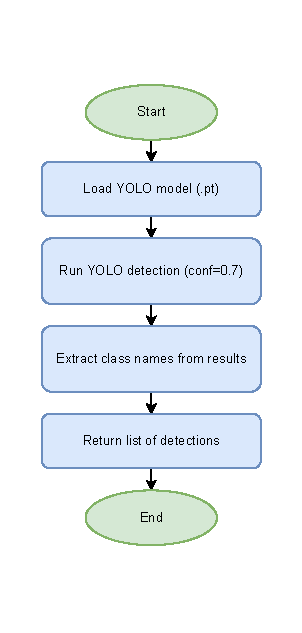
\includegraphics[width=0.3\textwidth]{Figures/diagrams/run_image_analysis.pdf}
    \caption{Process overview of image analysis function using the trained \gls{yolo}v11 model.}
    \label{run_image_analysis}
\end{figure}

The function runs the detection using the \texttt{predict} function provided by Ultralytics. As shown in Listing~\ref{lst:model_predict_only}, the trained model is first loaded from the \texttt{best.pt} file. Then, the \texttt{predict} method is called with the input image path and a confidence threshold of zero point seven. The \texttt{save} option is enabled to store the result image with the drawn bounding boxes. Additionally, the confidence value of zero point seven was selected to filter out low confidence detections and reduce the number of false positives. This value ensures that only predictions with a high certainty are considered during evaluation.

\begin{figure}
    \begin{lstlisting}[language=Python, caption={Running model prediction on a given image using Ultralytics functions}, label={lst:model_predict_only}]
        # Load the trained YOLO model
        model = YOLO("best.pt")
    
        results = model.predict(
            source=image_path,
            conf=0.7,
            save=True,
        )
    \end{lstlisting}
\end{figure}




\subsection{Data Flow And Processing Pipeline}

This subsection outlines the complete data flow and processing pipeline for the \gls{db} test environment. Figure~\ref{Complete_process} illustrates the entire workflow, showing the interaction between components and the flow of data throughout the test execution process.

\begin{figure}[!ht]
    \centering
    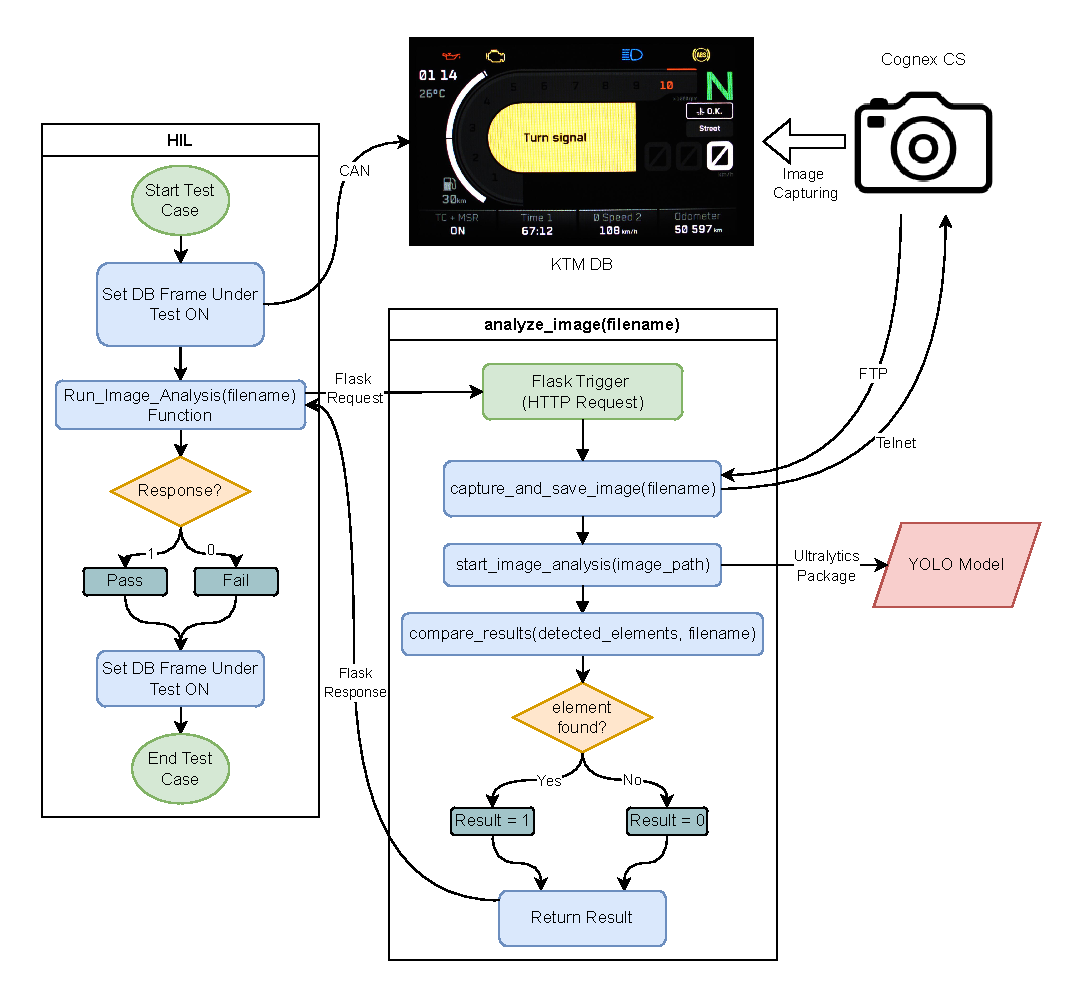
\includegraphics[width=\textwidth]{Figures/diagrams/Complete_Process (1).pdf}
    \caption{Overview of the complete data flow and processing pipeline used in the \gls{db} test environment.}
    \label{Complete_process}
\end{figure}

The interaction begins on the \gls{hil}, which starts the test case and sets the \gls{db} frame under test by sending the appropriate CAN messages. Once the frame is active, the \gls{hil} sends an HTTP request to the using Flask to the standalone \gls{sw} to trigger the \texttt{analyze\_image(filename)} function.

The request starts a sequence steps. First, the \texttt{capture\_and\_save\_image(filename)} function commands the \gls{cs} via \gls{telnet} to capture an image and download it to the directory using \gls{ftp}. The saved image path is then passed to the next function which is \texttt{start\_image\_analysis(image\_path)}, where the trained \gls{yolo} model is loaded and used to detect visible elements. Additionally, it extracts the elements names and add them to a list to simplifies the comparing process.

Next, the \texttt{compare\_results(detected\_elements, filename)} function compares the detected elements from the list with the expected elements indicated by the filename. If the elements are found, the function returns a value of one, otherwise, it returns zero. This result is sent back to the \gls{hil} through the Flask response to conclude the test case.

This process could then be used with differant combinations of \gls{db} telltale icons and run multiple times to perform a conclusive automated testing of this class in the \gls{db} \gls{sw}. Moreover, the results of running this test case is discussed in the results chapter. Additionally, the results of the model training and testing are also documented in the next chapter. 


